% вторая часть

\section{Анализ показаний приборов учета}

Учет и анализ коммунальных ресурсов дает возможность выявить их перерасход, вызванный, возможно, и халатным отношением, либо неисправностью сетей подачи ресурса. Также становится прозрачным перерасход ресурсов и несанкционированное их потребление.\cite{journal}

«Личный кабинет» программы СКАУТ позволяет получить часовые, суточные и ежемесячные данные в виде таблиц и графиков, что позволяет удобно анализировать расход ресурсов.

Детализация данных для всестороннего анализа.
Посуточная статистика. Пример приведен на рис.~\ref{fig:day}
\begin{figure}[H]
	\centering
	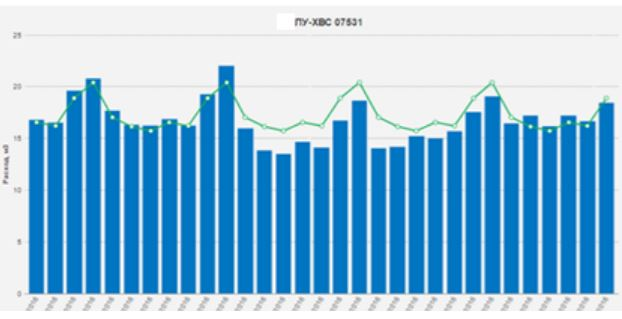
\includegraphics[width=0.7\linewidth]{pics/day}
	\caption{Посуточное потребление}
	\label{fig:day} 
\end{figure}
Почасовая статистика. Пример приведен на рис.~\ref{fig:hour}
\begin{figure}[H]
	\centering
	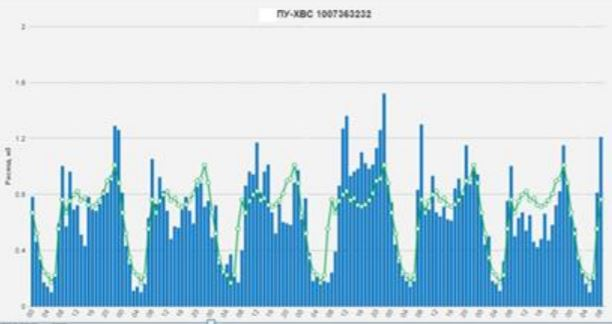
\includegraphics[width=0.7\linewidth]{pics/hour}
	\caption{Почасовые показания}
	\label{fig:hour} 
\end{figure}

С выведением информации по средне статическому потреблению.
Графическое представление, особенно за длительные сроки, даёт наглядную картину работы водосчетчиков и электросчетчиков. 

Несколько сложнее обнаруживать утечки в системе горячего водоснабжения. Непрерывный и неравномерный разбор горячей воды затрудняет их определение. Использование статистики потребления горячей воды жилым домом в ночные часы (3 часа ночи) позволяет улавливать фоновые потери для каждого дома. В основном это передавливание горячей воды в трубопровод холодного водоснабжения через неисправные квартирные смесители. Установив для каждого дома фоновый уровень потерь, можно контролировать появление протечек. До настоящего времени нами не было обнаружено таких протечек, однако данным методом в Обнинске были выявлены два 100 квартирных дома, где фоновое потребление холодной воды на дом достигало 600 литров
в час и более. В квартирах одного их них были обнаружены два неисправных сливных бачка, в другом доме протекал вентиль в подвале, и вода уходила в ливневую канализацию. После ремонтов фоновое потребление в этих домах установилось на уровне 250–300 литров в час. \cite{journal2}

Так же известно, что потребление горячей воды не может превышать потребление холодной. Данная проблема сигнализирует нам об неисправности счетчика. С помощью наложения двух графиков потребления горячей и холодной воды, можем наглядно увидеть проблемные счетчики.